\section{Ejercicio FR - Gráficas}

\subsection{Problema}

Represente la trayectoria de la partícula en el espacio tridimensional y analice los resultados.

Presente en una misma gráfica el comportamiento de tres velocidades adimensionales (extraídas de la anterior simulación) en función del tiempo medido en nanosegundos. En concreto, se pide el módulo de la velocidad del electrón relativista en función del tiempo, el componente $v_z$ de su velocidad y su velocidad radial $v_r = \sqrt{ v_x^2 + v_y^2}$. 

\subsection{Resolución}

El código que resuelve este ejercicio se puede ver en \ref{code:ex11}.

\paragraph{Gráfica de $\vec{r}(t)$} 
Primero mostramos los componentes de $\vec{r}(t)$ en función de $t$.

\begin{figure}[H]
	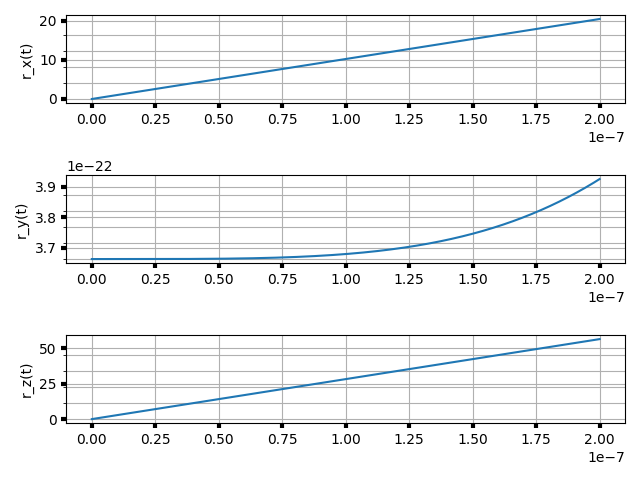
\includegraphics[width=\linewidth]{figures/rel_rx_ry_rz.png}
	\caption{Gráfica $r_x(t)$, $r_y(t)$, $r_z(t)$ en función de $t$}
	\label{fig:rel_rx_ry_rz_t}
\end{figure}

\newpage 

\paragraph{Gráfica en 3D de $\vec{r}(t)$} 
La trayectoria de la partícula en 3D.

\begin{figure}[H]
	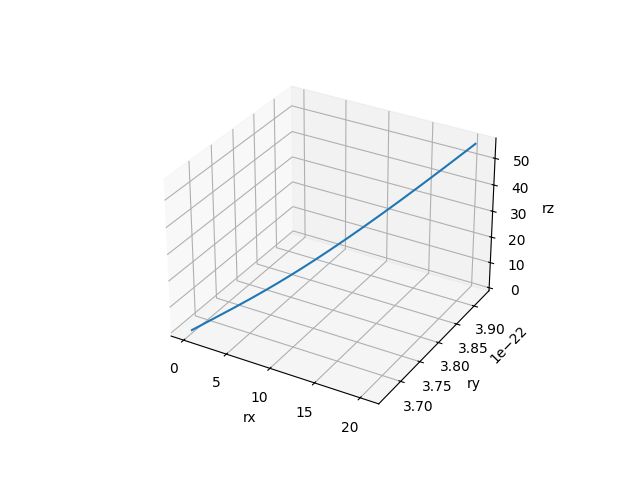
\includegraphics[width=\linewidth]{figures/rel_3d_r.png}
	\caption{Gráfica $r_x(t)$, $r_y(t)$, $r_z(t)$ en 3D}
	\label{fig:rel_3d_r}
\end{figure}

\newpage 

\paragraph{Gráfica de $\frac{\vec{v}(t)}{c}$}

La gráfica de los componentes de $\vec{v}(t)$ adimensionada por $c$.

\begin{figure}[H]
	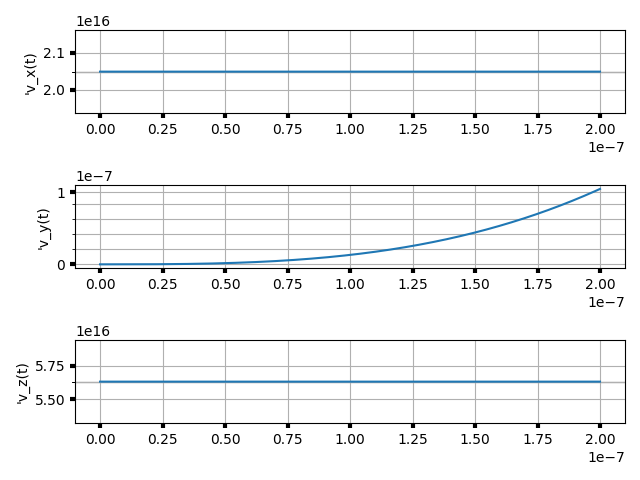
\includegraphics[width=\linewidth]{figures/rel_adim_vx_vy_vz.png}
	\caption{Gráfica $\vec{v}(t)$ adimensionada}
	\label{fig:rel_adim_vx_vy_vz}
\end{figure}

\newpage 

\paragraph{Gráfica de $||v||, v_{radial}$ y $v_z$} La gráfica de $||v||$, $v_r$ y $v_z$ (adimensionadas por $c$).

\begin{figure}[H]
	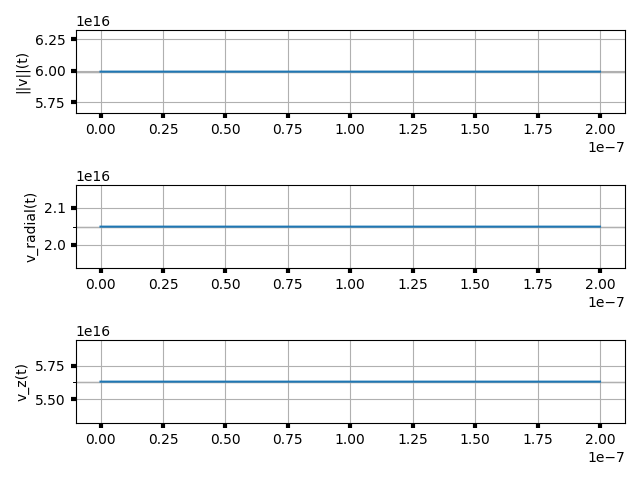
\includegraphics[width=\linewidth]{figures/rel_v_mod_rad_z.png}
	\caption{Gráfica $v_r$ y $v_z$}
	\label{fig:rel_v_radial_vz}
\end{figure}
